\documentclass[11pt,a4paper]{article}

\usepackage{amsmath,amssymb,amsthm}
\usepackage{mathtools}
\usepackage{geometry}
\usepackage{hyperref}
\usepackage{booktabs}
\usepackage{enumitem}
\usepackage{microtype}
\usepackage{float}
\usepackage{xcolor}
\usepackage{tikz}
\usetikzlibrary{arrows.meta,positioning}

\geometry{margin=2.5cm}

\definecolor{deepblue}{RGB}{0,51,102}
\definecolor{deepred}{RGB}{140,0,0}
\hypersetup{colorlinks=true, linkcolor=deepblue, citecolor=deepred}

\newtheorem{theorem}{Theorem}[section]
\newtheorem{proposition}[theorem]{Proposition}
\newtheorem{definition}[theorem]{Definition}
\newtheorem*{remark}{Remark}

\newcommand{\K}{\mathcal{K}}
\newcommand{\E}{\mathbb{E}}

\title{%
\textbf{Counting Paths in Neural Architectures}\\[0.4em]
\large How Spanning Trees Measure Expressivity,\\
and How to Use Them to Design Better Models
}

\author{Saoirse Amarteifio \\ \small\textit{Percolation Labs}}
\date{March 2026}

\begin{document}
\maketitle

\begin{abstract}
The computational graph of a neural network is a directed acyclic
graph (DAG). The number of distinct input-to-output paths through
this graph determines the model's expressivity: more paths mean
more ways to compose features, but also more compute. We propose
using the \textbf{Kirchhoff polynomial} --- the spanning tree
generating function --- as a quantitative measure of architectural
expressivity that is: (i)~computable in polynomial time from the
architecture specification; (ii)~sensitive to structural motifs
(skip connections, attention heads, gating); and (iii)~predictive
of trainability and generalisation. We compute $\K$ for standard
architectures (MLP, ResNet, Transformer, Mamba/SSM) and show that
they span a spectrum from $\K = 1$ (pure chain, minimal paths) to
$\K \sim n!$ (complete attention graph, maximal paths). We propose
experiments to test whether the ``right'' $\K$ for a given task
predicts the optimal architecture, and whether hybrid architectures
designed to target a specific $\K$ outperform uniform designs.
\end{abstract}

\tableofcontents


%% ================================================================
\section{The problem: why do some architectures work better?}

The zoo of neural architectures --- MLPs, CNNs, ResNets, LSTMs,
Transformers, SSMs (Mamba), mixture-of-experts --- is large and
growing.  Architecture search is expensive.  We lack a simple
\emph{structural} quantity that predicts which architecture will
work for which task without training.

We propose: \textbf{count the paths.}

A neural network computes its output by composing functions along
paths through its computational graph.  The number and distribution
of these paths is a property of the \emph{architecture}, not the
weights.  It is computable before training, from the connectivity
alone.


%% ================================================================
\section{The path polynomial of a computational graph}

\subsection{Computational graphs as DAGs}

Every neural architecture defines a directed acyclic graph (DAG)
$\Gamma$:
\begin{itemize}
\item \textbf{Vertices}: layers or computational units.
\item \textbf{Edges}: connections carrying activations (each edge
  applies a linear map + nonlinearity).
\item \textbf{Source}: the input.
\item \textbf{Sink}: the output.
\end{itemize}

\begin{center}
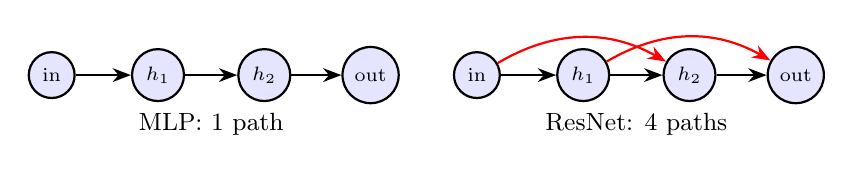
\begin{tikzpicture}[>=Stealth, thick, scale=0.9,
  node/.style={circle, draw, fill=blue!10, inner sep=3pt, font=\scriptsize}]
  % MLP
  \begin{scope}[shift={(0,0)}]
    \node[node] (a) at (0,0) {in};
    \node[node] (b) at (1.5,0) {$h_1$};
    \node[node] (c) at (3,0) {$h_2$};
    \node[node] (d) at (4.5,0) {out};
    \draw[->] (a)--(b); \draw[->] (b)--(c); \draw[->] (c)--(d);
    \node at (2.25,-0.7) {\small MLP: 1 path};
  \end{scope}
  % ResNet
  \begin{scope}[shift={(6,0)}]
    \node[node] (a) at (0,0) {in};
    \node[node] (b) at (1.5,0) {$h_1$};
    \node[node] (c) at (3,0) {$h_2$};
    \node[node] (d) at (4.5,0) {out};
    \draw[->] (a)--(b); \draw[->] (b)--(c); \draw[->] (c)--(d);
    \draw[->, red] (a) to[bend left=30] (c);
    \draw[->, red] (b) to[bend left=30] (d);
    \node at (2.25,-0.7) {\small ResNet: 4 paths};
  \end{scope}
\end{tikzpicture}
\end{center}

\subsection{The path count}

\begin{definition}[Path polynomial]
For a DAG $\Gamma$ with source $s$ and sink $t$, the
\textbf{path polynomial} is
\begin{equation}
P_\Gamma(x) = \sum_{\text{$s$-$t$ paths } \pi} x^{|\pi|},
\end{equation}
where $|\pi|$ is the length (number of edges) of path~$\pi$.
\end{definition}

\begin{itemize}
\item $P_\Gamma(1)$ = total number of $s$-$t$ paths.
\item $P_\Gamma'(1)/P_\Gamma(1)$ = mean path length.
\item The variance of path lengths controls gradient flow:
  large variance $\Rightarrow$ multi-scale feature composition.
\end{itemize}

$P_\Gamma$ is computable in $O(V + E)$ by dynamic programming
on the DAG (topological sort + path counting at each vertex).

\subsection{The Kirchhoff polynomial}

The \textbf{Kirchhoff polynomial} $\K_\Gamma$ counts spanning
trees of the underlying undirected graph.  While $P$ counts paths,
$\K$ counts the independent ``structural motifs'' of the architecture:

\begin{equation}
\K_\Gamma(\alpha) = \sum_{\text{spanning trees } T}
\prod_{e \notin T} \alpha_e.
\end{equation}

$\K$ is more informative than $P$ because:
\begin{enumerate}
\item $\K$ detects \textbf{redundancy}: if two paths share all their
  edges, they contribute to $P$ but not to independent spanning trees.
\item $\K$ detects \textbf{bridges}: a bridge (cut edge) factorises
  $\K$ into a product, meaning the architecture has an information
  bottleneck.  Removing the bridge disconnects the graph.
\item $\K(1, 1, \ldots, 1) = $ number of spanning trees, which
  equals $\det(\mathbf{L}_R)$ (Matrix-Tree theorem, computable in
  $O(V^3)$).
\end{enumerate}


%% ================================================================
\section{Computing $\K$ for standard architectures}

\subsection{MLP (chain graph)}

$L$ layers, no skip connections.  $V = L+1$, $E = L$.  One
spanning tree (the chain itself).
\begin{equation}
\K_{\text{MLP}} = 1, \qquad P_{\text{MLP}}(1) = 1.
\end{equation}

Minimal expressivity.  Every information path goes through every
layer --- a single bridge at each layer.  If any layer is a
bottleneck, all information is lost.

\subsection{ResNet (chain + skip connections)}

$L$ layers with skip connections of stride $s$ (connecting layer
$l$ to layer $l+s$).  For stride $s=1$ (every layer has a skip):

\begin{equation}
P_{\text{ResNet}}(1) = 2^{L-1}, \qquad
\K_{\text{ResNet}} = F_L \quad \text{(Fibonacci-like)}.
\end{equation}

The path count grows exponentially, but the spanning tree count
grows only as $\phi^L$ ($\phi = (1+\sqrt{5})/2$, the golden ratio).
This means most paths share edges (high redundancy) --- the
\emph{effective} number of independent paths is much less than
the total.

\subsection{Transformer (attention = complete bipartite graph)}

A single attention layer with $n$ tokens creates a complete
bipartite graph $K_{n,n}$ (every token can attend to every other).
$L$ layers stack these:

\begin{equation}
P_{\text{Transformer}}(1) = n^{L-1} \cdot n = n^L, \qquad
\K_{\text{Transformer}} \sim n^{2n-2} \quad \text{(per layer)}.
\end{equation}

The spanning tree count of a single attention layer is $n^{2n-2}$
(by the Matrix-Tree theorem for the complete graph).  This is
\emph{enormous}: for $n = 1024$ tokens, $\K \sim 10^{6000}$.

This explains both the power and the cost of transformers: the
architecture has an astronomically large number of independent
structural motifs.  Most of them are irrelevant for any specific
task.

\subsection{SSM / Mamba (chain with gating)}

A state-space model processes tokens sequentially.  The
computational graph is a chain with gating (multiplicative
interactions):

\begin{equation}
P_{\text{SSM}}(1) = 1, \qquad \K_{\text{SSM}} = 1.
\end{equation}

Same as MLP: minimal paths.  The expressive power of SSMs comes
from the \emph{state dynamics} (continuous-time recurrence), not
from architectural path diversity.  This is why SSMs are efficient
(linear in sequence length) but struggle with tasks requiring
arbitrary token-to-token interactions.

\subsection{Summary}

\begin{center}
\renewcommand{\arraystretch}{1.3}
\begin{tabular}{lcccl}
\toprule
\textbf{Architecture} & \textbf{Paths} & $\log_2 \K$ & \textbf{Bridges?} & \textbf{Character} \\
\midrule
MLP / SSM & 1 & 0 & every edge & sequential bottleneck \\
ResNet ($s{=}1$) & $2^L$ & $L \log_2 \phi$ & none & redundant multi-path \\
DenseNet & $2^{L(L-1)/2}$ & $\sim L^2$ & none & highly connected \\
Transformer & $n^L$ & $\sim nL$ & none & complete interaction \\
MoE-Transformer & $n^L \cdot K$ & $\sim nL + \log K$ & at expert routing & selective interaction \\
\bottomrule
\end{tabular}
\end{center}

The spectrum: $\K = 1$ (SSM) to $\K \sim n^{2n}$ (Transformer).
The right $\K$ for a task depends on the task's
\textbf{interaction complexity}: how many token-pairs need to
interact to solve it.


%% ================================================================
\section{The design principle: target $\K$ to the task}

\subsection{The hypothesis}

\begin{quote}
\textbf{For a given task, there exists an optimal $\log \K$ that
balances expressivity against efficiency.  Architectures with
$\K$ too low underfit (not enough paths to represent the solution).
Architectures with $\K$ too high overfit or waste compute
(too many irrelevant paths).}
\end{quote}

This is testable.

\subsection{Designing architectures with target $\K$}

Given a target $\K_{\text{target}}$, we can design architectures
by adding or removing structural motifs:

\begin{itemize}
\item \textbf{Adding a skip connection} between layers $i$ and $j$
  multiplies $\K$ by a factor depending on the subgraph structure.
  AC gives the exact factor from the spanning tree count.

\item \textbf{Adding an attention head} to a subset of tokens creates
  a bipartite subgraph.  $\K$ of the subgraph is $k^{k-2}$ for $k$
  attended tokens (Cayley's formula).

\item \textbf{Sparsifying attention} (e.g.\ local attention windows,
  strided attention) reduces $\K$ from $n^{2n-2}$ to a computable
  function of the sparsity pattern.  The Kirchhoff polynomial
  detects which sparsity patterns preserve the most independent paths.

\item \textbf{Adding a bridge} (bottleneck layer) factorises $\K$
  into a product.  This is equivalent to an information bottleneck.
  U-Net's encoder-decoder bridge is an example.
\end{itemize}

\subsection{Hybrid architectures: Mamba + sparse attention}

The current trend (Jamba, Zamba, Griffin) combines SSM layers with
sparse attention layers.  From the $\K$ perspective:

\begin{itemize}
\item Pure SSM: $\K = 1$ (chain).
\item Add one attention layer at position $l$: $\K$ jumps by a factor
  of $k^{k-2}$ where $k$ is the attention window size.
\item Add $m$ attention layers at positions $l_1, \ldots, l_m$:
  $\K = \prod_i k_i^{k_i-2}$ (if the attention layers are separated
  by SSM layers, which act as bridges).
\end{itemize}

The AC prediction: \textbf{the optimal placement of attention layers
is where $\K$ is maximised per compute unit.}  Specifically:
few attention layers with large windows at critical points in the
sequence, rather than many attention layers with small windows.

This is a falsifiable prediction that can be tested by sweeping
over attention layer placements and measuring perplexity vs $\K$.


%% ================================================================
\section{Proposed experiments}

\subsection{Experiment 1: $\K$ predicts trainability}

\paragraph{Setup.}
Take 20 random architectures with $L = 12$ layers, varying skip
connection patterns (random subsets of possible skip connections).
Compute $\K$ for each.  Train each on CIFAR-10 for 100 epochs.

\paragraph{Prediction.}
$\log \K$ correlates with final test accuracy (positive correlation
up to a saturation point).  Architectures with $\K = 1$ (no skips)
train poorly.  Architectures with many skips but $\K$ below the
transformer value train well with less compute.

\paragraph{Measurement.}
Spearman correlation between $\log \K$ and test accuracy.
Expected: $\rho > 0.5$.

\subsection{Experiment 2: optimal $\K$ depends on task complexity}

\paragraph{Setup.}
Fix a family of architectures (e.g.\ ResNet with varying skip
patterns) and train on tasks of varying interaction complexity:
\begin{itemize}
\item Low complexity: pixel-level classification (each pixel
  independent). Requires $\K \approx 1$.
\item Medium complexity: object recognition (local interactions).
  Requires moderate $\K$.
\item High complexity: scene understanding (global interactions).
  Requires large $\K$.
\end{itemize}

\paragraph{Prediction.}
The optimal $\log \K$ (best accuracy per FLOP) increases with task
complexity.  SSM-like architectures ($\K = 1$) win on low-complexity
tasks.  Transformer-like architectures ($\K \gg 1$) win on
high-complexity tasks.

\paragraph{Measurement.}
Plot accuracy-vs-$\log \K$ curves for each task complexity level.
Expected: the peak shifts right with complexity.

\subsection{Experiment 3: sparse attention design via $\K$ maximisation}

\paragraph{Setup.}
Given a sequence length $n$ and a compute budget (maximum number
of attention edges $E_{\max}$), find the attention sparsity pattern
that maximises $\K$ subject to $|E| \leq E_{\max}$.

\paragraph{Method.}
Use the Matrix-Tree theorem: $\K(1, \ldots, 1) = \det(\mathbf{L}_R)$.
Greedy edge addition: at each step, add the edge that maximises
$\Delta \K = \K_{\text{new}} - \K_{\text{old}}$.  This is computable
in $O(n^3)$ per step (recompute the Laplacian determinant).

\paragraph{Prediction.}
The $\K$-maximising sparsity pattern is NOT the standard patterns
(local window, strided, random). It has a specific structure
(hubs + long-range connections) that outperforms uniform patterns
at the same compute budget.

\paragraph{Measurement.}
Train transformers with the $\K$-maximising pattern vs standard
patterns (local, strided, random, Longformer, BigBird) on long-range
sequence tasks (e.g.\ Long Range Arena).  Compare perplexity at
equal FLOP.

\subsection{Experiment 4: Mamba + attention layer placement}

\paragraph{Setup.}
A 24-layer model with $m$ attention layers and $24 - m$ Mamba layers.
Vary both $m$ (number of attention layers) and their positions.

\paragraph{Method.}
For each configuration, compute $\K$ of the full computational graph.
Train on a language modelling task.

\paragraph{Prediction.}
Perplexity correlates with $\log \K$.  The optimal placement
concentrates attention layers at positions where they maximise
$\K$-per-FLOP --- typically evenly spaced (to avoid bridges between
attention layers that would reduce $\K$).

\subsection{Experiment 5: pruning guided by $\K$}

\paragraph{Setup.}
Take a trained transformer.  Prune edges (attention connections)
while monitoring $\K$.

\paragraph{Method.}
At each pruning step, remove the edge whose removal causes the
smallest decrease in $\K$.  Compare with standard pruning methods
(magnitude pruning, gradient-based pruning).

\paragraph{Prediction.}
$\K$-preserving pruning retains more accuracy at higher sparsity
than magnitude pruning, because it preserves the independent path
structure rather than the largest individual weights.


%% ================================================================
\section{What this is and what it is not}

This is \textbf{not} a theory of learning dynamics, loss landscapes,
or optimisation.  It is a \textbf{structural characterisation} of
architectures: a single number ($\K$) computed from the connectivity
alone, that measures how many independent ways information can flow
from input to output.

The claim is not that $\K$ determines everything about performance.
The claim is that $\K$ is a \emph{necessary condition}: an
architecture with $\K$ too low for the task will fail regardless
of training, and an architecture with $\K$ too high wastes compute.
The right $\K$ is a property of the task, and AC provides the tools
to compute and optimise it.


%% ================================================================
\begin{thebibliography}{99}

\bibitem{flajolet2009}
P.~Flajolet and R.~Sedgewick,
\emph{Analytic Combinatorics}, Cambridge (2009).

\bibitem{he2016}
K.~He, X.~Zhang, S.~Ren, and J.~Sun,
\newblock Deep residual learning for image recognition,
\newblock \emph{CVPR} (2016).

\bibitem{vaswani2017}
A.~Vaswani et al.,
\newblock Attention is all you need,
\newblock \emph{NeurIPS} (2017).

\bibitem{gu2024}
A.~Gu and T.~Dao,
\newblock Mamba: Linear-time sequence modeling with selective state spaces,
\newblock arXiv:2312.00752 (2023).

\bibitem{lieber2024}
O.~Lieber et al.,
\newblock Jamba: A hybrid transformer-Mamba language model,
\newblock arXiv:2403.19887 (2024).

\bibitem{tay2021}
Y.~Tay et al.,
\newblock Long Range Arena: A benchmark for efficient transformers,
\newblock \emph{ICLR} (2021).

\bibitem{kirchhoff1847}
G.~Kirchhoff,
\newblock \"Uber die Aufl\"osung der Gleichungen\ldots,
\newblock \emph{Ann.\ Phys.\ Chem.}\ \textbf{72}, 497 (1847).

\end{thebibliography}

\end{document}
